\documentclass{beamer}

\usetheme{Madrid}
\usecolortheme{whale}

\usepackage{xcolor}
\usepackage{etoolbox}
\usepackage{ifthen}

\usepackage{tcolorbox}
\tcbuselibrary{skins,xparse}
% \tcbuselibrary{listings}
% \tcbuselibrary{minted}
% \tcbset{listing engine=minted}

\usepackage{graphicx}
\usepackage{hyperref}
\usepackage{listings}

% Bib configs
\usepackage[backend=biber, sorting=none]{biblatex}
\addbibresource{refs.bib}
\DeclareFieldFormat*{title}{#1}
\DeclareFieldFormat*{url}{\newline\url{#1}\nopunct}
\DeclareFieldFormat{labelnumberwidth}{#1\adddot}
\setlength{\biblabelsep}{5pt}
\renewcommand*{\bibfont}{\tiny}
\usepackage{ragged2e}

% cmd: urls in .bib
\newcommand{\biburl}[2][]{%
\newline - \ifstrempty{#1}{}{\textcolor{cyan}{#1: }}\url{#2}\nopunct
}

% cmd: Ask and answer tcolorbox
\newcommand{\askanswer}[5]{ % title, note, [You], Ask,Bing AI, Answer
  \begin{tcolorbox}[
    title=#1,
    skin=bicolor,
    colframe=black,
    colbacklower=green!10,
    fontupper=\small,
    fontlower=\footnotesize,
    middle=0pt, % Remove space of \tcblower
    subtitle style = {
      boxrule=0.4pt,
      colback=gray,
    }
  ]
    #2
    \tcbsubtitle{You}
    {\color{blue} #3}
    \tcblower
    \tcbsubtitle{#4}
    #5
  \end{tcolorbox}
}

\usepackage{datetime}
\yyyymmdddate % 2023/05/08

\title{GPT Survey: A Programmer's Perspective}
\author{Yu Zehan}
\institute{Intel FLEX}
\date{\today}

% cmd: Lesson template with: section, title, toc
\newcounter{lesson_cnt}
\newcommand{\lesson}[1]{
  \stepcounter{lesson_cnt}
  \section{Lesson \arabic{lesson_cnt}: #1}
  \subtitle{Lesson \arabic{lesson_cnt}: #1}
  \begin{frame}
    \titlepage
  \end{frame}
  \begin{frame}{Outline of Lesson \arabic{lesson_cnt}}
    % \tableofcontents[currentsection,hideothersubsections]
    \tableofcontents[sections={\arabic{lesson_cnt}}]
  \end{frame}
}

\begin{document}

\begin{frame}
  \titlepage
\end{frame}

\begin{frame}{Outline}
  \tableofcontents[hideallsubsections]
\end{frame}

% Lesson 1
\date{2023/05/09}
\lesson{Prompt Engineering: Principles, Techniques, and Tools}

\subsection{SPQA Architecture}
\begin{frame}{SPQA Architecture}
  \centering
  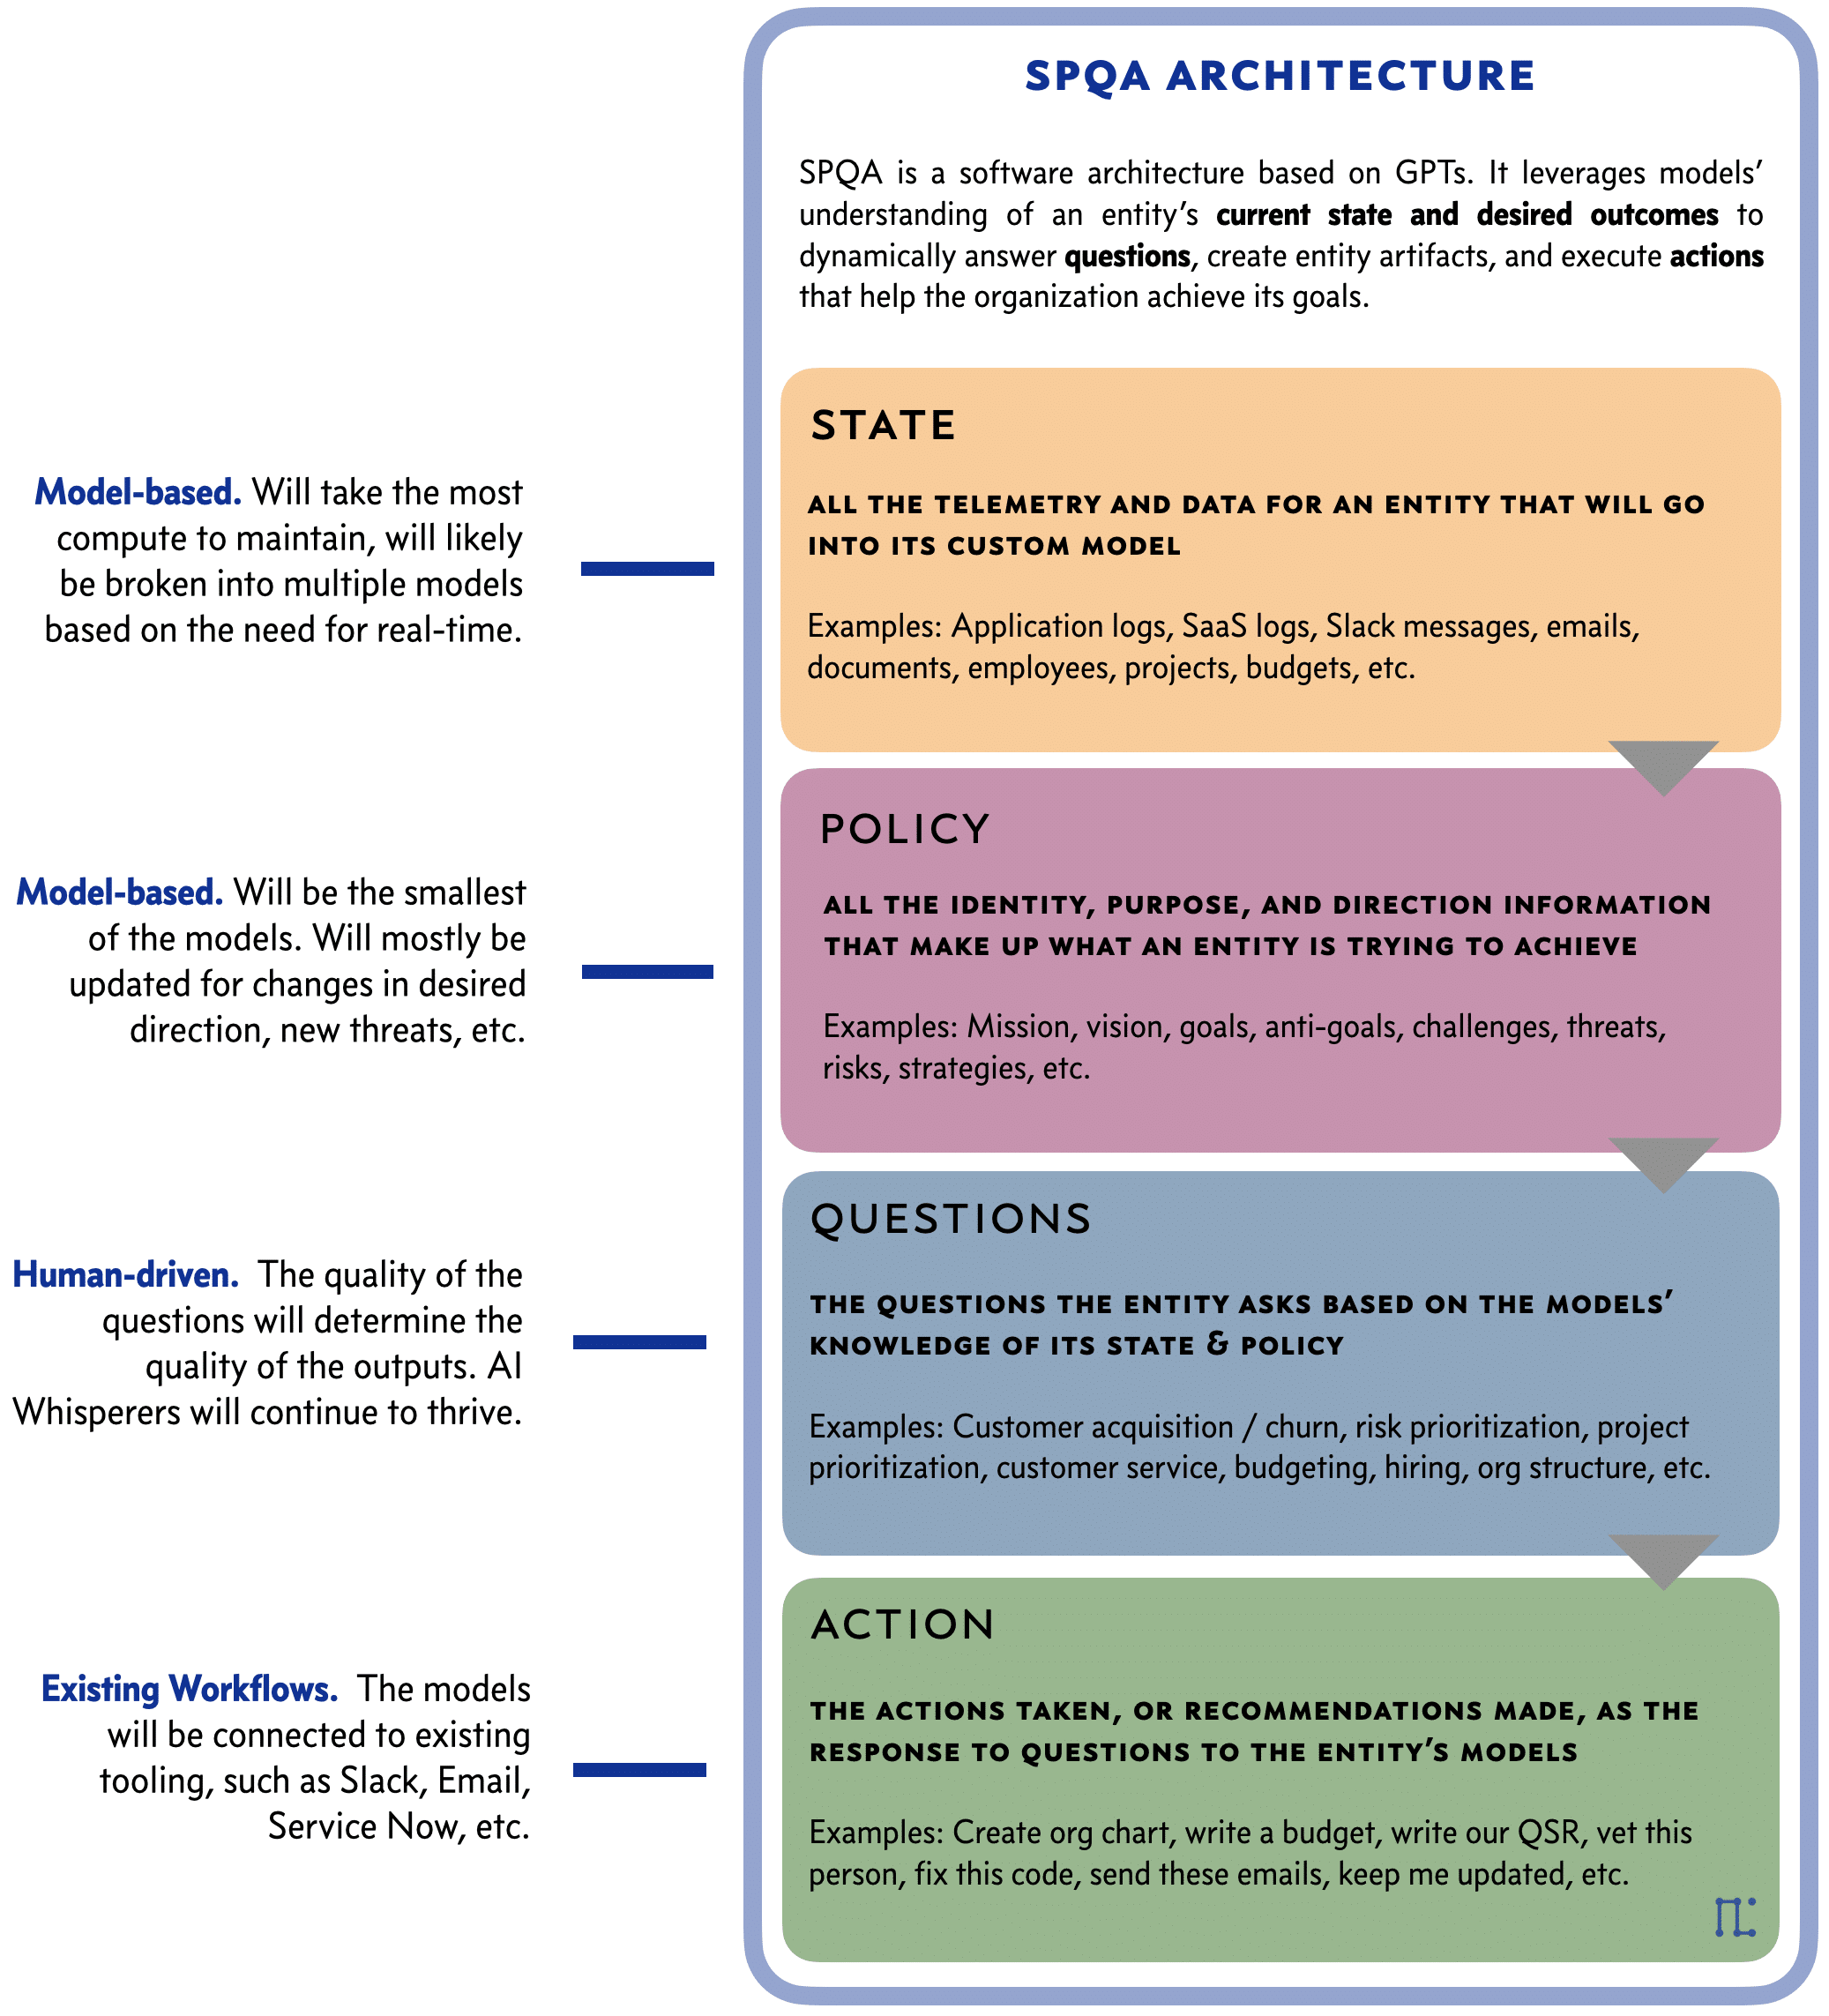
\includegraphics[width=\linewidth,height=0.8\textheight,keepaspectratio]{./images/spqa-3-architecture-model-based.png}
\end{frame}

\begin{frame}{Circuit-Based vs Understanding-Based}
  \centering
  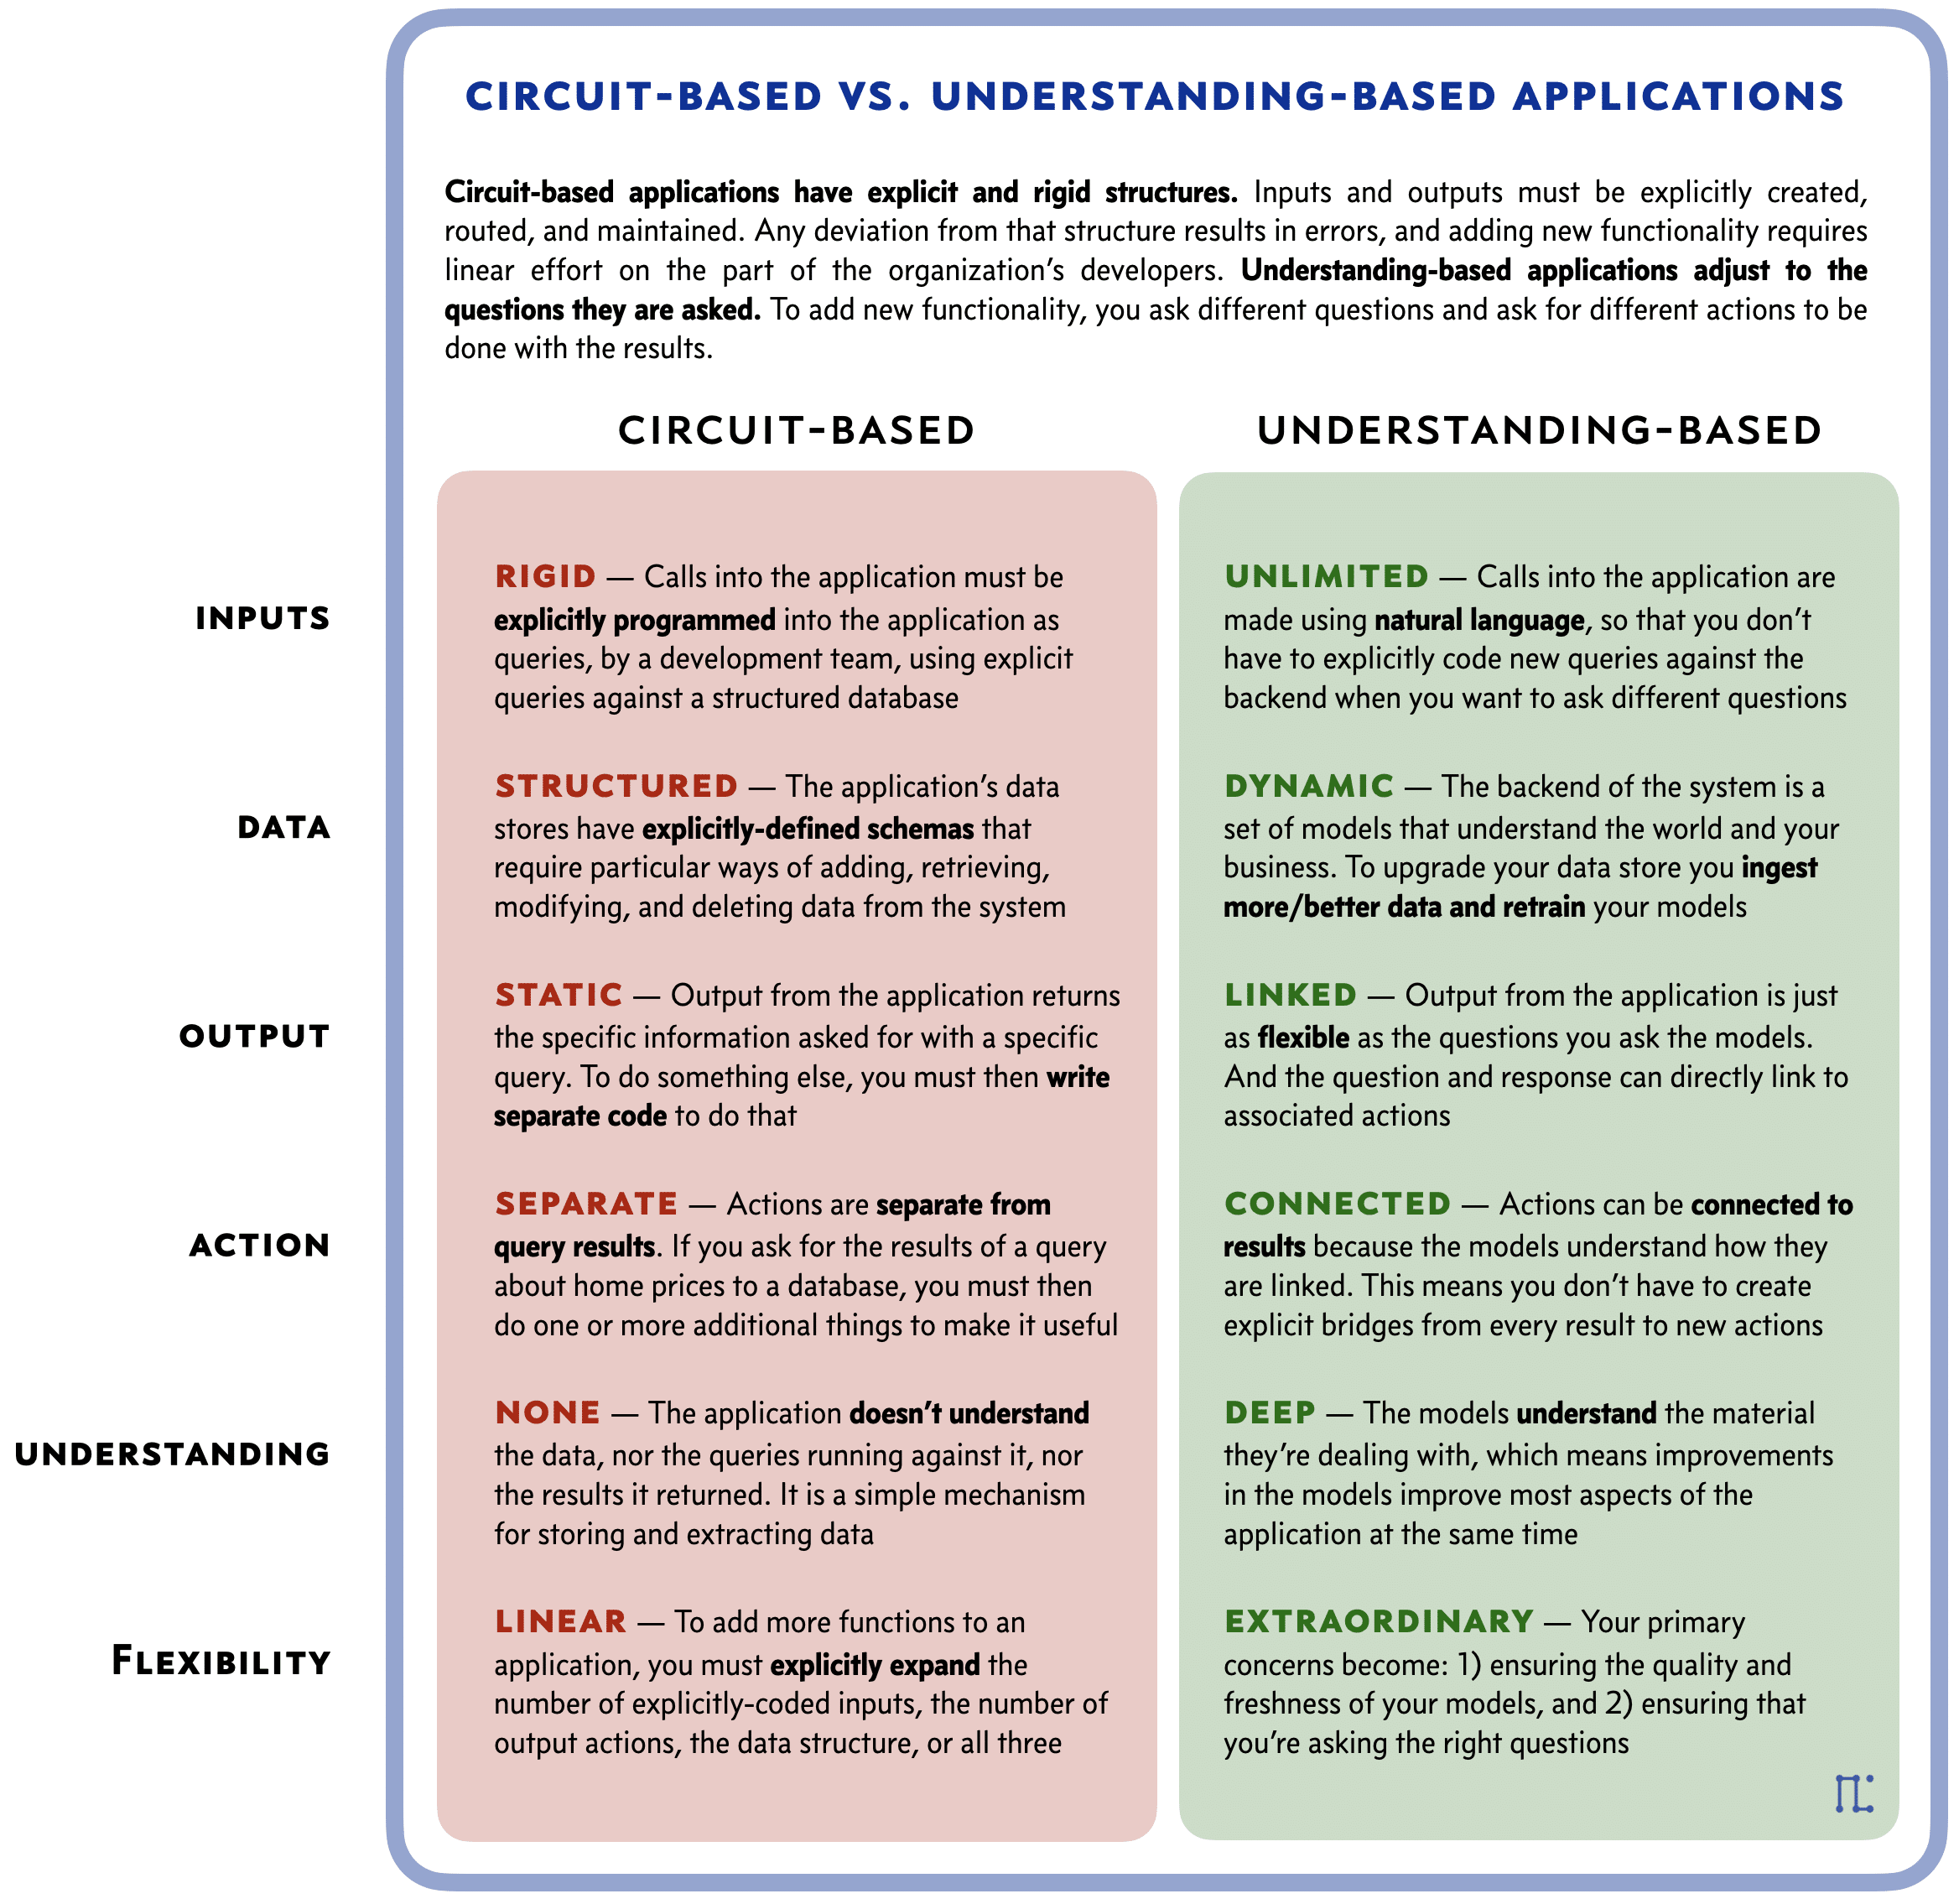
\includegraphics[width=\linewidth,height=0.8\textheight,keepaspectratio]{./images/spqa-1-circuit-vs-understanding.png}
\end{frame}

\subsection{Prompt Workflows}
\begin{frame}{Prompt Workflows}
  \centering
  \begin{minipage}[c][\textheight][c]{0.38\linewidth}
    \vspace{-3\topskip}
  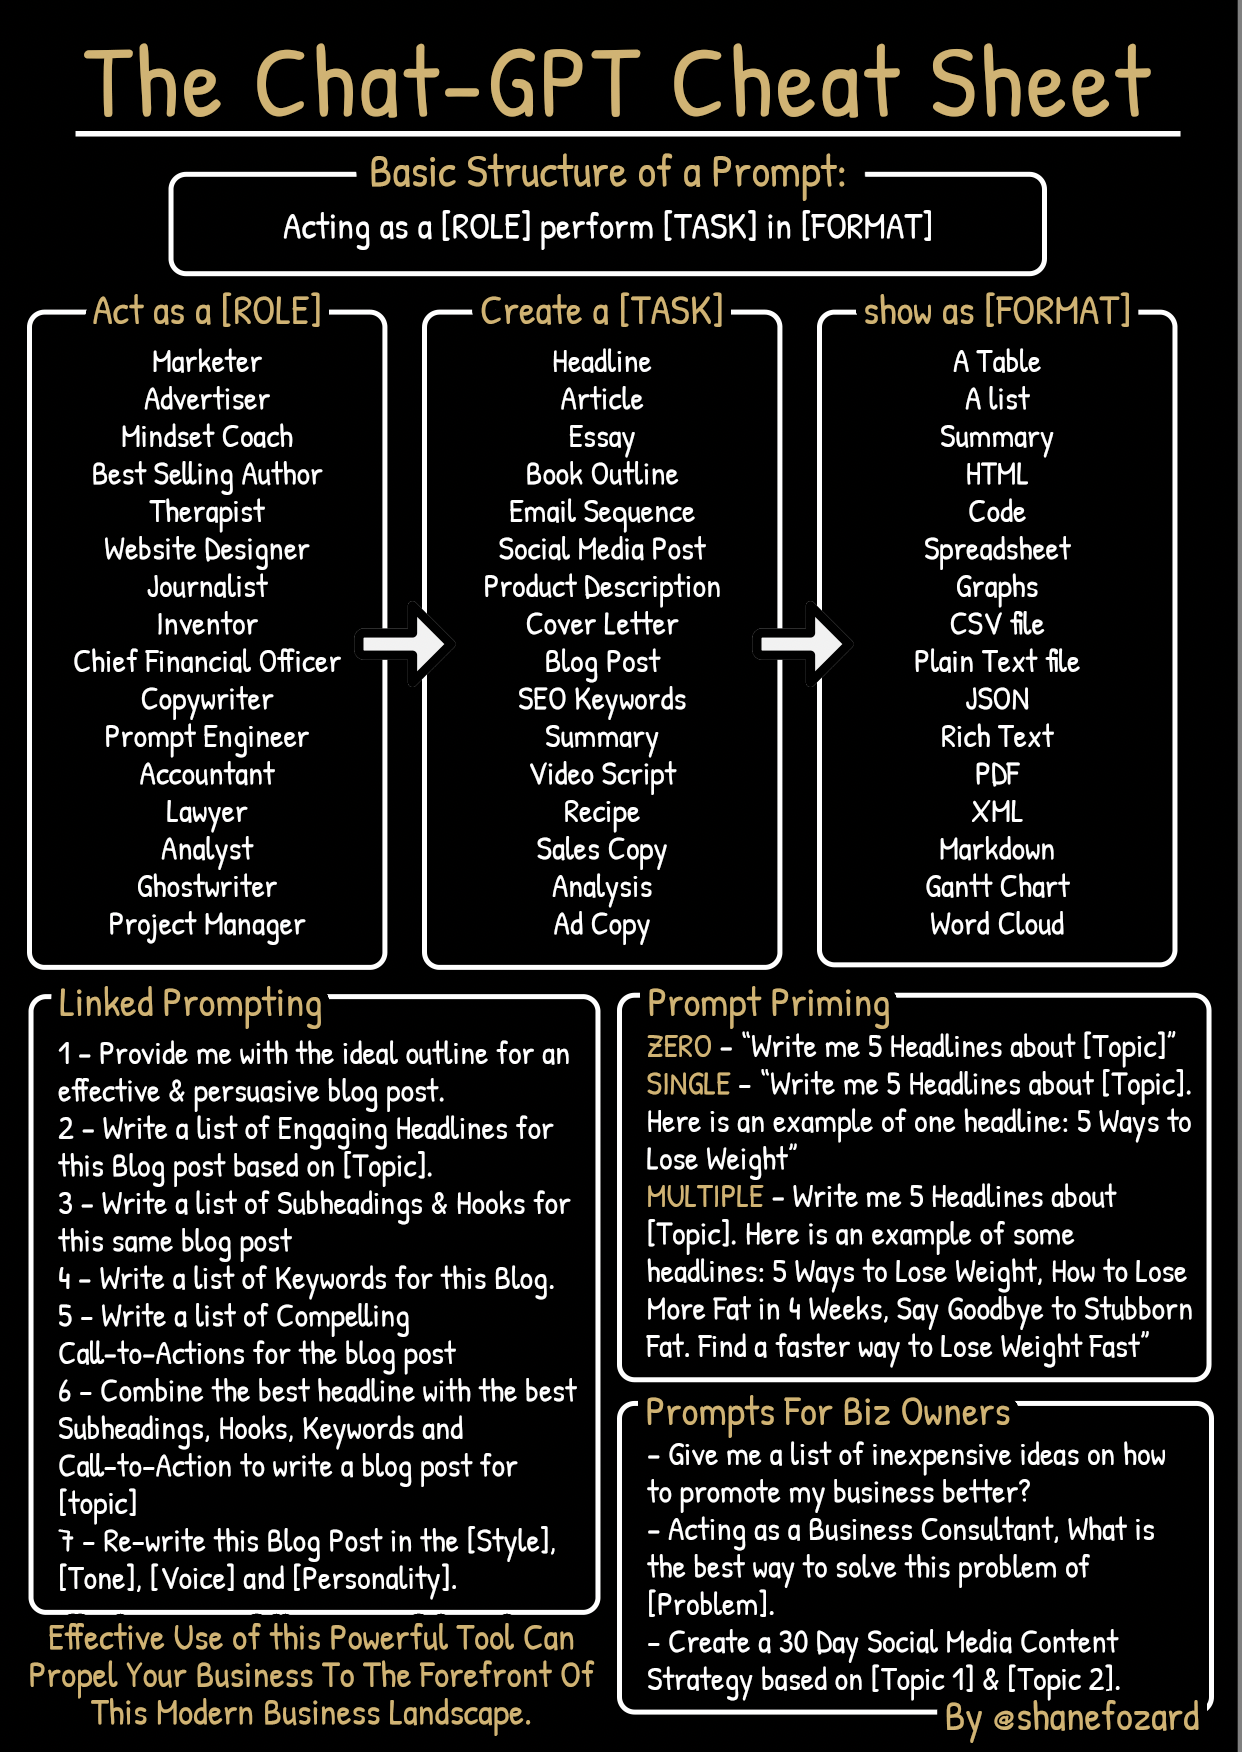
\includegraphics[width=\linewidth,keepaspectratio]{./images/chatgpt-cheatsheet.png}
  \end{minipage}
  \hfill
  \begin{minipage}[c][\textheight][c]{0.18\linewidth}
    \vspace{-3\topskip}
  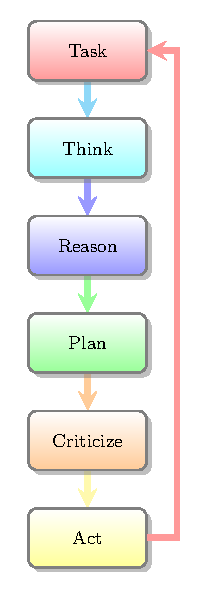
\includegraphics[width=\linewidth,keepaspectratio]{./tikz-prompt-workflow-autogpt.pdf}
  \end{minipage}
  \hfill
  \begin{minipage}[c][\textheight][c]{0.32\linewidth}
    \vspace{-3\topskip}
    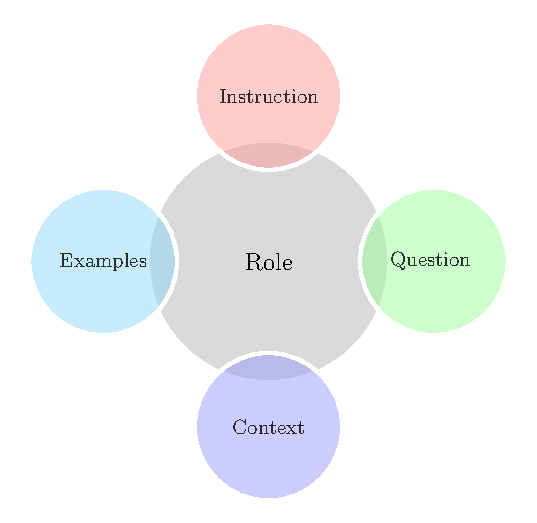
\includegraphics[width=\linewidth,keepaspectratio]{./tikz-prompt-workflow-common.pdf}
  \end{minipage}
\end{frame}

\subsection{Prompt Principles}
\begin{frame}{Prompt Principles}
% More details and examples
  % One-shot or Few shots
% Structured
  % Delimiters
  % Formatted instructions and examples
% Iterate
  % Step by step
  % self-check
% Top to Bottom
  % Divide and conquer

  \centering
  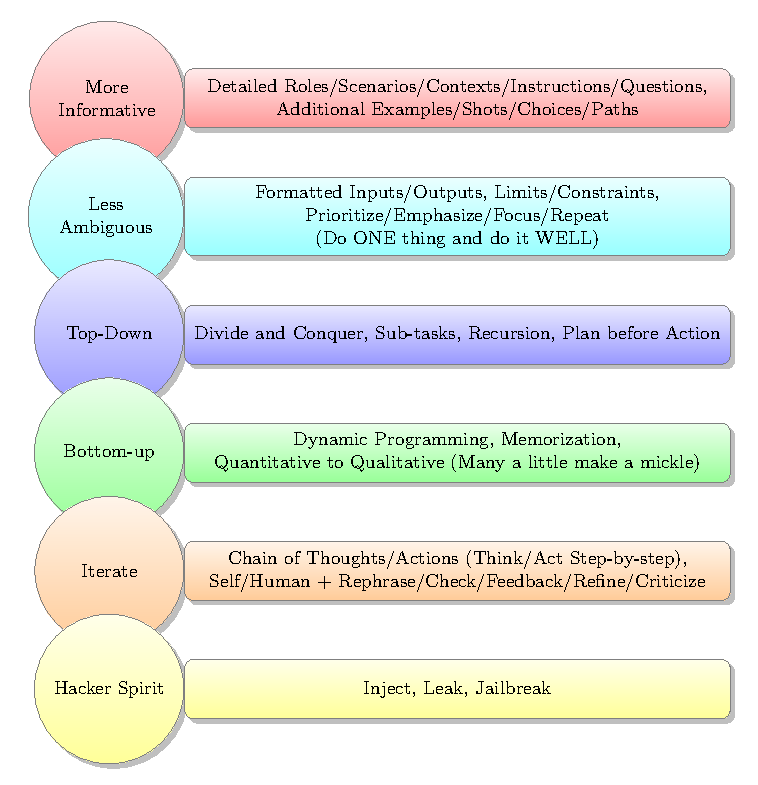
\includegraphics[width=\linewidth,height=0.8\textheight,keepaspectratio]{./tikz-prompt-principles.pdf}

  % More details
  % Do One Thing And Do It Well (DOTADIW)
  % Iteration 
  % Shots
  % Structured Inputs and Outputs
  % Search Engine is still powerful
\end{frame}

\subsection{Prompt Techniques}
\begin{frame}{Prompt Techniques: Let's Start!}
  \askanswer{A Hello World Case}
  {Here is where we start.}
  {Write a Scrawler for me.}
  {Bing AI}
  {I’m sorry, but I’m not able to write a web scraper for you. However, I can provide you with information on how to write one yourself or where to find resources to learn how to do so. Would you like me to help you with that?}
\end{frame}

\begin{frame}{Prompt Techniques: Little change makes huge effects}
  \askanswer{Little change makes huge effects}
  {Add programming language; Use Scraper that AI understood.}
  {Provide a Python Scraper script.}
  {Bing AI}
  {Here is a basic Python script that can be used as a starting point for writing a web scraper:
  
  ... {\color{green!50!black} (\# Python codes Here)}
  %     import requests
  %     from bs4 import BeautifulSoup
      
  %     url = 'https://www.example.com' # Replace with the URL you want to scrape
  %     page = requests.get(url)
  %     soup = BeautifulSoup(page.content, 'html.parser')
      
  %     # Find the data you want to scrape using BeautifulSoup methods
  %     data = soup.find_all('div', class_='example-class')
      
  %     # Process the data as needed
  %     for item in data:
  %         print(item.text)

  This script uses the `requests` and `BeautifulSoup` libraries to fetch and parse the HTML of a web page. You can then use the methods provided by `BeautifulSoup` to find and extract the data you want from the page.
  
  Keep in mind that this is just a basic example and you may need to modify it to fit your specific needs. Additionally, make sure to follow any terms of service or usage policies for the website you are scraping.}

\end{frame}
%   % Use delimiters
%   % Ask for structured output
%   % Instruct the model to check conditions
%   % Use few-shot prompting.

\begin{frame}{Prompt Techniques: More Infromative}
  \centering
  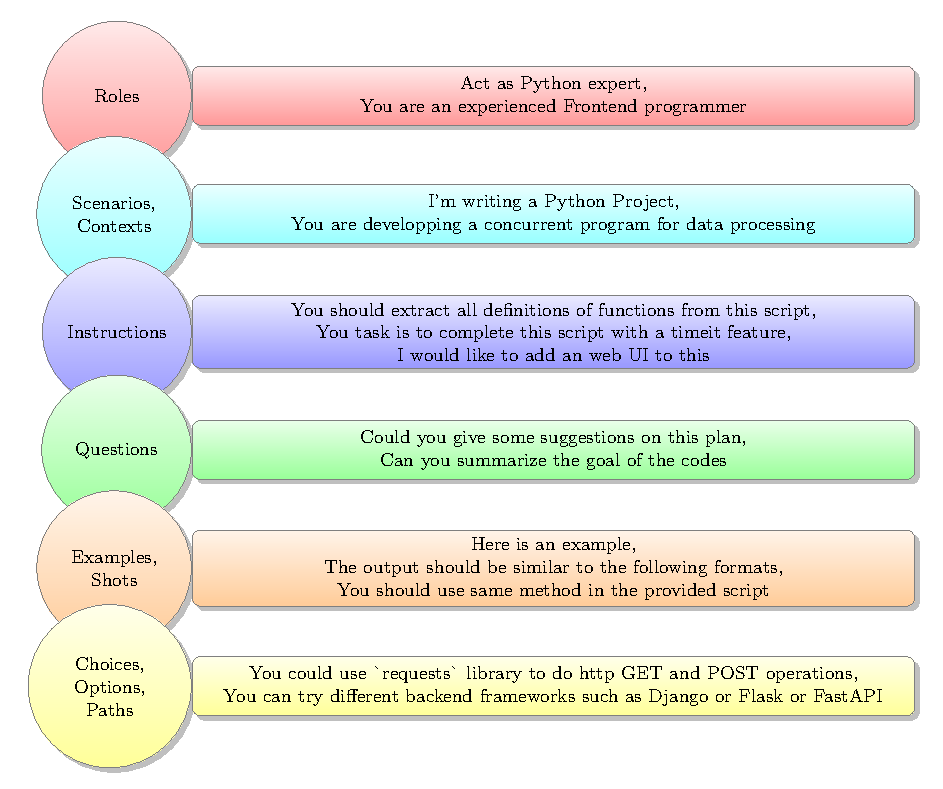
\includegraphics[width=\linewidth,height=0.8\textheight,keepaspectratio]{./tikz-prompt-techniques-more-informative.pdf}
\end{frame}

\begin{frame}{Search Engine is Still Your Friend}
\end{frame}

\begin{frame}{Human Skills is Still Important}
\end{frame}

\subsection{Tools and Extensions}
\begin{frame}{GPT applications comparisons}
  
\end{frame}

\begin{frame}{Tools and Extensions}
  
\end{frame}

% Lesson 2
\date{2023/05/15}
\lesson{Integrate GPT in Whole Coding Lifecycle}
\begin{frame}
\titlepage
\end{frame}

% Lesson 3
\lesson{Cutting-Edge GPT Projects and Showcases}
\begin{frame}
  \titlepage
\end{frame}

% Lesson 4
\lesson{Customize GPT for More Power}
\begin{frame}
\titlepage
\end{frame}

\begin{frame}
\end{frame}


\section{References}
\begin{frame}[t,allowframebreaks]{References}
  \nocite{*}
  \RaggedRight
  \printbibliography
\end{frame}


\begin{frame}{FAQ}

\end{frame}

\end{document}
